\label{sec:abc_dt}

A typical \abcpt{} follows a traditional compiler's structure:

\begin{enumerate}
  \item \textbf{Parse \abc{} input}\\ \hfill
    The \abc{} parser generates an internal representation (\ac{IR}) to be transformed in the
    following stage.
  \item \textbf{Transform the generated representation}\\ \hfill
    The \ac{IR} is transformed.
  \item \textbf{Generate the output}\\ \hfill
    An output of the transformed \ac{IR} is generated.
\end{enumerate}

Figure \ref{fig:process_stages} illustrates an \abcpt{}'s architecture.

\begin{figure}[H]
  \centering
  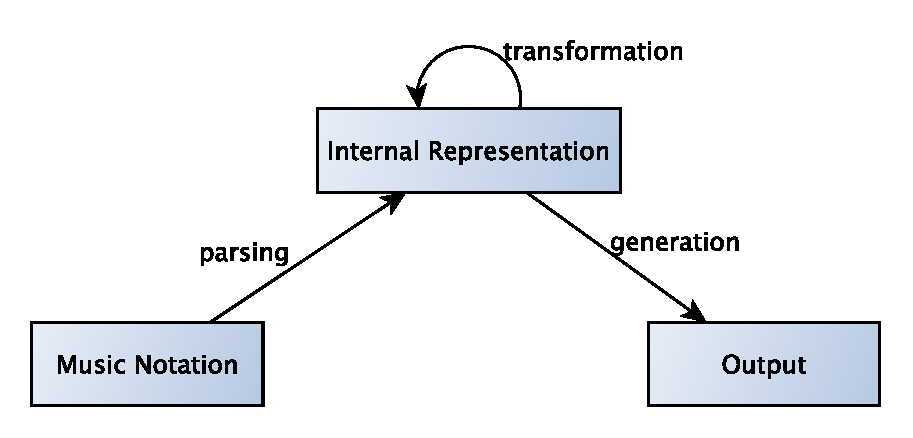
\includegraphics[width=0.8\textwidth]{img/abc_dt.pdf}
  \caption{\abcpt{}'s architecture}
  \label{fig:process_stages}
\end{figure}

In order to be able to create new \abcpt{}s in the most simple and compact way possible, a \ac{DSL}
called \abcdt{} was created as well as its processor, in which:

\begin{enumerate}
  \item The parsing process is invoked automatically, considering the parser is constant and
  independent of the intended transformation, thus being common to every \abcpt{}.
  \item The \ac{IR}'s transformation is described by a set of rules specified by the user (referred
  to as \abcdtrules{}). Each rule is composed by the pair \emph{actuator $\Rightarrow$
  transformation}, where the \actuator{} describes the \ac{IR}'s part to be processed and the
  \transformation{} is the set of instructions to be applied to that part.
  \item The output generation in \abc{} format is provided by default. The default function is the
  identity function - \toabc{}.
\end{enumerate}

The details of \abcdt{}'s implementation will be described next, following the three stages of the
architecture aforementioned.

\section{Parse ABC Input}
\label{sec:parse}

As was previously stated in the introduction, an \abcpt{} must be able to deal with real \abc{}
music. Therefore, the \abc{} parser has to be robust, i.e., it must be able to expect cases that it
doesn't recognize.

The main options for building the parser were: to build it from scratch; to reuse an existing parser
from robust programs like \abcmtops{}~\cite{abcm2ps:Online} or \abctomidi{}~\cite{abc2midi:Online}
and adapt it to the requirements; or to use directly one of the aforementioned programs' parsers.

Since building a robust parser is very time consuming, the first solution was discarded. The second
option would raise problems when adapting it to newer versions. So, using \abcmtops{} or
\abctomidi{}'s parser was the natural choice. The program chosen was \abcmtops{} for the reasons
that are explained in the following section.

\subsection{\abcmtops{} parser's features}

\abcmtops{} is one of the most widely used programs for working with \abc{}, not just as a
standalone software but as part of many applications. This fact implies that it's not a piece of
software that was casually made. It was designed to process \abc{} in the best way possible,
therefore its quality is acknowledged.

It is actively maintained and well documented which facilitates the analysis of the structures its
parser generates. Moreover, its author, Jeff Moine, was and still is a preponderant influence for
the evolution of the \abc{} notation and standard. Its parser is also used in other Moine's tools
like \tclabc{}~\cite{tclabc:Online}.

The \ac{IR} generated by its parser follows the sequential structure type and it's \sourcewise{}. In
other words, each element captured by the parser is simply appended to an ordered list, resulting in
a sequence of \abcelements{} in the same order they are parsed. An element is any component existing
in \abc{}, from the header information - like the key or initial meter - to a note, bar, a tuplet or
lyrics.

Given that \abcmtops{} was designed to print \abc{} scores, its \ac{IR} (\sourcewise{}) is not well suited
for music analysis or composition purposes. Still, it can be easily transformed into different views
of the same representation. For instance, a \timewise{} \ac{IR} could be a set of monophonic voices,
which could be used to describe relationships between vertical musical entities on a polyphonic
score.

% Therefore, it lacks all the benefits inherent to an hierarchical
% representation, such as, inheriting behavior and characteristics between musical events.
As the aim of this dissertation is to build a toolkit based on scripts, the sequential structure is
very appropriate since the sequence of elements that it provides can be easily mapped to an
\emph{array} or a \emph{hash}. These data types are part of the common, yet powerful, data types of
a scripting language like Perl, which is the kind of approach that's intended.

\subsection{From \abcmtops{} parser's IR to Perl}

At this point, it was necessary to define a strategy to implement the first stage (\emph{Parse
\abc{} Input}).

It consists in selecting the best and most robust tool that processes \abc{}, isolate its parser and
finally add a traversal function that serializes\footnote{Serialization is the process of
translating data structures into a format that can be stored and resurrected later in the same or
another computer environment.} the \ac{IR}'s structure so that it can be evaluated by Perl into a Perl
structure.

Perl is the developing language being used and, since it supports reflection\footnote{Reflection is
the ability of a computer program to examine and modify the structure and behavior (specifically the
values, meta-data, properties and functions) of an object at runtime.}, it provides the ability to
evaluate a string as if it were a source code statement at runtime.

So \abcmtops{} is the tool selected to have the parser extracted. Its parser is implemented in C, so
the structure that it generates is a list of C data structures. Therefore, a C program - called
\abctoperl{} - was created. It uses \abcmtops{}' parser to parse an \abc{} file into a C structure,
then it translates that structure into a serialized Perl \emph{hash} which is then printed to the
standard output.

In short, \emph{Parse \abc{} Input} stage is comprised of a Perl serialization of the structure
generated by \abcmtops{}' parser (\abctoperl{}), followed by a Perl evaluation of the serialized
structure into a Perl \emph{hash}. This way, a Perl structure that maps the original C structure is
obtained, which can be manipulated in the following stages.

Figure \ref{fig:parse_abc_input_stage} depicts the internal workflow of \emph{Parse \abc{} Input}
stage. \abctoperl{}'s workflow is represented by the group node '\abctoperl{}'.

\begin{figure}[htb]
  \centering
  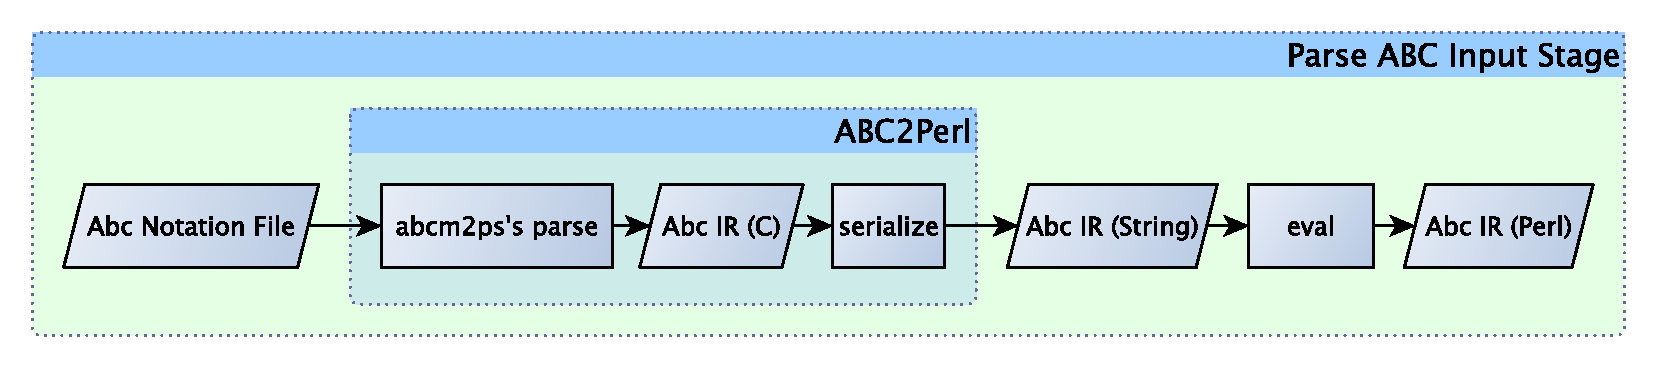
\includegraphics[width=\textwidth]{img/parse_abc_input_stage.pdf}
  \caption{\emph{Parse \abc{} Input} stage}
  \label{fig:parse_abc_input_stage}
\end{figure}

A simple mapping of the original C structure into a Perl one is being made. Hence the original order
and meaning are being kept. However, it could be possible to reorganize the structure to serve other
purposes. For example, representing it by part (\partwise{}) means that a specific part can be
accessed directly. Or representing it by elapsed time (\timewise{}) means that it is be possible to
directly retrieve all musical events that occur in a specific moment in time.

The approach being used in this strategy can be reused in other situations similar to this one where
a parser is needed and there already exists a powerful one. \abcdt{}'s parser update process is
facilitated due to its constituents being autonomous, which means that only those constituents need
to be updated to newer versions.

An Haskell specification of the serialized structure can be consulted in appendix
\ref{sec:abcm2ps_parser_ir}.

\section{Transform the generated representation}

This stage consists of making a traversal of the \ac{IR} generated in the previous stage and
applying a rule-based transformation to it.

The generic processing strategy is based on a structured processing of the \ac{IR}. It is possible
to process complex structures, like \abcmtops{}', if its processing is divided , i.e., if there are
many small surgical transformations done to its parts, and each individual result is composed into a
single one.  This approach has been successfully used, for instance, in the processing module of XML
documents, XML::DT~\cite{tesejj}, attribute grammars~\cite{paakki1995attribute} and
\emph{Stratego}~\cite{Stratego:Online}.  This strategy is called DT (\emph{Down Translate}) and it's
basically a depth traversal of the structure where each individual element may have a specific
transformation associated.

The global transformation consists in specifying a set of rules. Those rules associate smaller
transformations to very specific points in the \ac{IR} and any point not covered in the rules is
kept unchanged, triggering the default transformation.

In order to provide a systematic and efficient method to specify the rules, a \ac{DSL} called
\abcdt{} was created. It allows the user to specify, in Perl, the rules to be applied to an \abc{}
score. It's actually a Perl module that can be seen as a \ac{DSL} embedded in Perl. The set of rules
is called \abcdtrules{}.

In the following sections, \abcdt{}'s main processor algorithm (\dt{}) and \abcdtrules{} are going
to be explained in more detail.

\subsection{Processor Algorithm}

\abcdt{}'s main processor is called \dt{}. It admits an \abc{} file which is parsed using the
\abctoperl{} program described in the previous section. It also admits a table of \abcdt{} rules - a
dispatch table\footnote{A dispatch table is a table of pointers to functions or methods.} - in which
an \actuator{} is associated with a \transformation{}.

It performs a traversal guided by the \ac{IR} meaning that a full traversal is done and each \abc{}
element is processed sequentially. Each visited element is matched against the table of \abcdt{}
rules in order to find the \transformation{} to apply. Additionally, the \context{} for the current
element is calculated, which consists of the voice's id and name, the time elapsed until that
element, the meter, the key, among others. The \context{} grants a more complete control of what can
be processed, thus providing a richer semantic processing.

It's possible to define a default transformation to cover any \abcelement{} that doesn't match any
rule. This is achieved through the rule \emph{-default}. Moreover, if no default transformation is
explicitly defined, then there is the default's default transformation, which is the identity
function (\toabc{}).

\dt{}'s behavior resembles the one from the utility \awk{}\footnote{\awk{} is a pattern scanning and
processing language, typically used as a data extraction and reporting tool}~\cite{awk:Online}
considering that the latter's processing is based on a sequence of pattern-action statements. Each
processed file is transformed into a sequence of symbols. Each symbol is processed one at a time and
matched against all patterns, and for each pattern that matches, the associated action is executed.
In \abcdt{}'s case, only the most specific \actuator{} (pattern) has its \transformation{} executed.
This is explained in more detail in section \ref{sec:abcdt_rules}.

\dt{}'s default output is the concatenation of each individual \transformation{}'s result, which is a
string. Optionally, a \emph{-end} rule can be added to the rules which enables a general post
processing of the final result, hence, making possible to attain different output formats.

The algorithm just described is expressed in Algorithm \ref{alg:dt}.

\begin{algorithm}
  \KwIn{abc-file}
  \KwIn{rules: $[(actuator,transf)]$}
  $musicIR \gets$ abc2perl(abc-file) \hfill //parse\\
  \ForAll{$ elem \in musicIR $}{
     $context \gets$ recalculate current context\\
     $transf\gets \mbox{rule ∈ rules with best matching actuator \textbf{or} -default \textbf{or} \toabc{}}$\\
     $res \gets res$ ++ $transf(elem, context)$ \\
  }
  \Return{rules[-end] \textbf{or} $res$}
  \caption{\dt{}'s algorithm}
  \label{alg:dt}
\end{algorithm}

The rule-based structured processing strategy grants an easy and effective way to build tools that
make simple transformations, considering that most of the processing is done in the background, this
is, it's only needed to provide the description of what is to be changed.

% In order to define how the outcome of processing a symbol should be merged with others, the
% processor must know which processing strategy it must use. Thus, a table of strategies is needed
% and by default the processor uses the \texttt{STR} strategy which makes the string concatenation
% of the outcome of each symbol.\\
% Other strategies might be added to the table. For instance, a strategy that maps a set of
% symbols to a Perl structure so that it can be processed as a whole. Such a set might be
% difficult to process with the default strategy.

\subsection{ABC::DT Rules}
\label{sec:abcdt_rules}

A language with the ability to do descriptive/surgical processing, in the sense that a
transformation may be applied to a specific element, enhances the effectiveness of the tool to be
generated. That ability takes shape as an \abcdt{} rule. It is a correspondence between an
\actuator{} and a \transformation{}.

\subsubsection{Actuator}

\emph{Actuators} act as a query language for selecting specific \abcelements{} (e.g.: a note) or a
set of elements (e.g.: all elements that are defined in a particular context/state). They are
designed in a way that there is a natural notation for matching (testing whether or not an \abc{}
element matches a pattern).

An \actuator{} (pattern) specifies a set of conditions on an \abcelement{}. An element that
satisfies the conditions matches the pattern; an element that does not satisfy the conditions does
not match the pattern.

There's an undirected graph of \abcelements{} that guides the pattern matching process. That graph
dictates the priority an \actuator{} has over other \actuators{}, so that if there's more than one
match, the most specific \actuator{}'s \transformation{} is applied to the \abcelement{}. Figure
\ref{fig:pscom} illustrates the graph for the \emph{pscom} class, in which the \actuators{}
\emph{MIDI} and \emph{FORMAT} are both instances of \emph{pscom} and therefore are more specific.
\emph{Actuator} \emph{MIDI::channel}\footnote{\emph{MIDI::channel} is an abcMIDI command that
selects a melody channel (ranging from 1 to 16 channels)} is an instance of \emph{MIDI} and is more
specific than the previous \actuators{}. Example \ref{ex:pscom_example} shows an example of the
\emph{actuator matching} process' behavior when facing a situation where there are more than one
possible matches.\\

\begin{figure}[h!]
  \centering
  \graph
  [scale=0.7]{g1}
  {
    margin="0 0 0 0";
    pscom--MIDI
    MIDI--"MIDI::channel"
    MIDI--"..."
    pscom--FORMAT;
    FORMAT--staves;
    FORMAT--autoclef;
    FORMAT--"....";
  }
  \caption{ Undirected graph of the \emph{pscom} class }
  \label{fig:pscom}
\end{figure}

\begin{program}
  An \abc{} element representing the abcMIDI command \emph{\%\%MIDI channel} is being subject to
  the \actuator{} matching process.\\

  The set of rules passed to the processor contains the \actuators{} \emph{pscom}, \emph{MIDI} and
  \emph{MIDI::channel}.\\

  The \abcelement{} satisfies the conditions specified by all of the \actuators{}, therefore the
  most specific has to be chosen.\\

  The graph dictates that the most specific \actuator{} is \emph{MIDI::channel}, so it is the
  actuator selected.

  \caption{\emph{Actuator matching}}
  \label{ex:pscom_example}
\end{program}

An \actuator{} is comprised of one to three components, each separated by the characters
'\emph{::}'.

An \actuator{} with just a single component represents either: 1) an \abc{} state, 2) an
\abcelement{} type, 3) a specific \abcelement{}, or 4) one of the special \actuators{}
(\emph{-default} and \emph{-end}).

\begin{enumerate}
  \item The \abc{} state represents the context in which an \abcelement{} appears in the tune. It
  can be \emph{in\_global} (any element written between the tune's beginning and the header
  \texttt{X:}), \emph{in\_header} (any element written between the headers \texttt{X:} and
  \texttt{K:}), \emph{in\_tune} (any element written after the header \texttt{K:}) and
  \emph{in\_line} (any embedded element, i.e. written between the characters '[' and ']').

  \item The \abcelement{} type represents a class of elements, such as \emph{note} (a note or a
  chord), \emph{info} (any \abc{} header (\texttt{K:}, \texttt{V:}, ...)), \emph{pscom} (any
  formatting or abcMIDI command), \emph{tuplet} (an element that indicates that the following
  elements belong to a tuplet), \emph{gchord}, \emph{deco} (respectively, an accompaniment chord and
  a decoration/ornament which are associated with a \emph{note}, \emph{rest} or \emph{bar}).

  \item A specific \abcelement{} represents an instance of a class of \abcelements{}, such as
  \emph{staves} (an instance of the class \emph{pscom}; it's a particular formatting command),
  \emph{!ff!} (an instance of the class \emph{deco}; it's a dynamics, \emph{fortissimo}), \emph{V:}
  (an instance of the class \emph{info}; it's the header that indicates that the following music
  belongs to the voice specified).

  \item The special \actuator{} \emph{-default} describes how to transform uncovered \abcelements{}
  and the \actuator{} \emph{-end} enables a general post processing of \dt{}'s final result, hence,
  making possible to attain different output formats.
\end{enumerate}

An \actuator{} may have other components added: 1) an instance of an \abcelement{}'s class, 2) a
restriction on \abcelements{}.

\begin{enumerate}
  \item An instance of an \abcelement{}'s class may be added, such as \emph{MIDI::channel}
  (\emph{channel} is an instance of \emph{MIDI} (abcMIDI command)) or \emph{note::C}
  (\emph{C} is an instance of \emph{note}).

  \item A restriction (filter) on \abcelements{} may be added, such as \emph{V:Tenor::rest} (it
  selects any \emph{element} \emph{rest} that belongs to the voice with name \texttt{Tenor}),
  \emph{bar::gchord::FINE} (selects any \emph{gchord} with text \texttt{FINE} that is associated to
  a \emph{bar}) or \emph{in\_line::K:} (selects all \emph{K:} \emph{elements} whose \emph{state} is
  \emph{in\_line}, this is embedded headers).
\end{enumerate}

Due to the existence of different levels of detail, when an \abcelement{} matches more than one
\actuator{}, the most specific is the one chosen. This corresponds to the deepest selectable node in
the graph of \actuators{}.

A list of the currently available \actuators{} in \abcdt{} rules may be consulted in appendix
\ref{sec:abcdt_rules_actuators}.\\

In the future, another approach to \actuators{} specification is going to be investigated. What's
intended is a richer syntax for identifying \abcelements{}, one that uses path expressions to
navigate through an \abc{} tune and has a set of standard functions to help selecting
\abcelements{}. This approach should be very similar to \emph{XPath}'s\cite{XPath:Online}.

\subsubsection{Transformation}

A \transformation{} is specified by the user and it defines how each \abcelement{} should be
processed according to its internal values.

\abcdt{} requires that only \abcelements{} that need to be transformed are specified, meaning that
what is not explicitly specified also needs to be processed. The default function which processes
the latter is the identity function - \toabc{} - and it prints the contents of an \emph{element}
just as it was in the \abc{} source file. \toabc{}'s Perl implementation was inspired on
Jean-François Moine's \tclabc{}~\cite{tclabc:Online} \symdumpi{} function which dumps the original
\abcelement{}.  \abcmtops{} and \tclabc{} use the same parser and \ac{IR}, therefore \symdumpi{}
integration in \abcdt{} was made without major obstacles.

In addition to user specified functions, there is a set of default functions that help accomplish
certain tasks which would otherwise make more difficult the creation of \abcpt{}s.
Music21~\cite{music21:Online} has been developing a set of effective methods for music processing
which reveal an advanced state of maturity, therefore they have been a source of inspiration for
some of the created functions.

Most of these functions emerged from simple necessity when some of the \abcpt{}s (described in
chapter \ref{chap:abc_dt_by_example}) were being built . Many \transformations{} were becoming very
complex and were making the code very hard to read and maintain, therefore, some functionalities
being implemented became \abcdt{} default functions. Some of those functions may be consulted in
appendix \ref{sec:abcdt_functions}.

As was previously mentioned in this section, during \dt{}'s traversal, for every \abcelement{}
visited, the \context{} is calculated. This \context{} allows the user to access contextual
information of the tune at that moment. It includes the current voice's \emph{id} and \emph{name},
the \emph{time} elapsed until that moment, the \emph{meter}, the total duration a measure should
have (\emph{wmeasure}), the note's \emph{length}, and the \emph{key} along with some properties: the
number of sharp/flats (\emph{sf}), the \emph{exp} flag, the number of explicit accidentals
(\emph{nacc}), the \midi{} number for each explicit note in the key element (\emph{pits}) and the
code that identifies the accidental for each explicit note in the key element (\emph{accs}).

\subsection{ABC::DT's main features}

\abcdt{}'s main features are summarized as follows:

\begin{description}
  \item[Dispatch Table] \hfill \\
    \abcdt{} rules are defined by a correspondence between the \actuators{} and \transformations{}.
  \item[Rich Actuators] \hfill \\
    The set of \actuators{} is comprised of well structured elements in order to provide a precise
    \abcelements{} matching.
  \item[Higher-Order Processing] \hfill \\
    The \transformations{} are user specified functions, or the identity function (\toabc{}).
  \item[Systematic] \hfill \\
    In order to build an \abcpt{}, the user must define what and how is to be transformed.
  \item[Specify only the necessary] \hfill \\
    If no \actuator{} applies, the \emph{default} function is used.
  % \item[Processing strategies] \hfill \\
  %   There is a table of strategies. Each strategy defines how a transformation's output is to be
  %   merged with others.
\end{description}

\section{Generate the output}

In this stage, an output of the transformed \ac{IR} is produced.

By default, \toabc{} is the transformation applied to an \abcelement{}, therefore the output
generated consists in the string concatenation of the individual transformations, which is
\abcdt{}'s universal type, the \abc{} stream.

The \abc{} stream is not the only format that can be generated as it depends on the intended purpose
for the \abcpt{} being built. \abcdt{} allows a post processing to be done at the end of the
\ac{IR}'s traversal, thus enabling a anything to be done with the intermediate transformations. This
is achieved through the \actuator{} \emph{-end} that has already been described earlier in this
chapter.

This control over the final format allows an \abcpt{} to be integrated with others that can make use
of the information generated.\\

Next, an hypothetical situation (meaning that the features described are not yet implemented in
\abcdt{}) where the graph format is used to help visualize characteristics present in a score that
are otherwise difficult to observe is described.

\subsection*{Note distribution by pitch and duration}

The purpose of the graph generated is to study the distribution of notes in a score, i.e., to find
correlations between pitch and duration. It plots three features: pitch, duration of notes, and how
frequently these pitches and durations are used.

\subsubsection*{Algorithm}

The algorithm used in this example consists in processing a tune with \dt{} in order to produce the
desired graph.

For every note found, the number of occurrences of the pair \emph{pitch $\Rightarrow$ duration} is
updated. In the end of \dt{}'s traversal, a post processing for generating the graph is done by
calling an auxiliar function that makes use of the note distribution data gathered during the
traversal and an external plotting tool, such as \emph{gnuplot}~\cite{gnuplot:Online},
Ti\emph{k}Z~\cite{tikz:Online}, \emph{Maxima}~\cite{maxima:Online}.

Table \ref{tab:plot_rules} describes an example of \abcdtrules{} that could be used with \dt{} in
order to generate the required graph.

\begin{center}
  \begin{table}[H]
    \begin{tabular}{|p{2.25cm}|p{7.25cm}|p{5cm}|}
      \hline
      Actuator & Transformation (Perl) & Notes\\
      \hline
      \hline
      \multirow{8}{*}{\emph{note}}
      & \$pitch = get\_pitch\_name(); & \emph{get\_pitch\_name()} is an \abcdt{} function that
      returns the note's pitch.
      \\

      & \$dur = get\_note\_length(); & \emph{get\_note\_length()} is an \abcdt{} function that
      returns the note's duration/length.
      \\

      & \$occurrence\{\$pitch\}\{\$dur\}++; & \emph{\%occurrence} stores the number of
      occurrences.
      \\
      \hline

      \hline
      \emph{-end} & plot(\%occurrence); & \emph{plot} would be an \abcdt{} function that given a
      structure like \emph{\%occurrence} generates a 3D graph.
      \\
      \hline
    \end{tabular}
    \caption{\abcdtrules{} for the graph generation}
    \label{tab:plot_rules}
  \end{table}
\end{center}

The graph generated is shown in figure \ref{fig:note_distribution}.

\begin{figure}[htb]
  \centering
  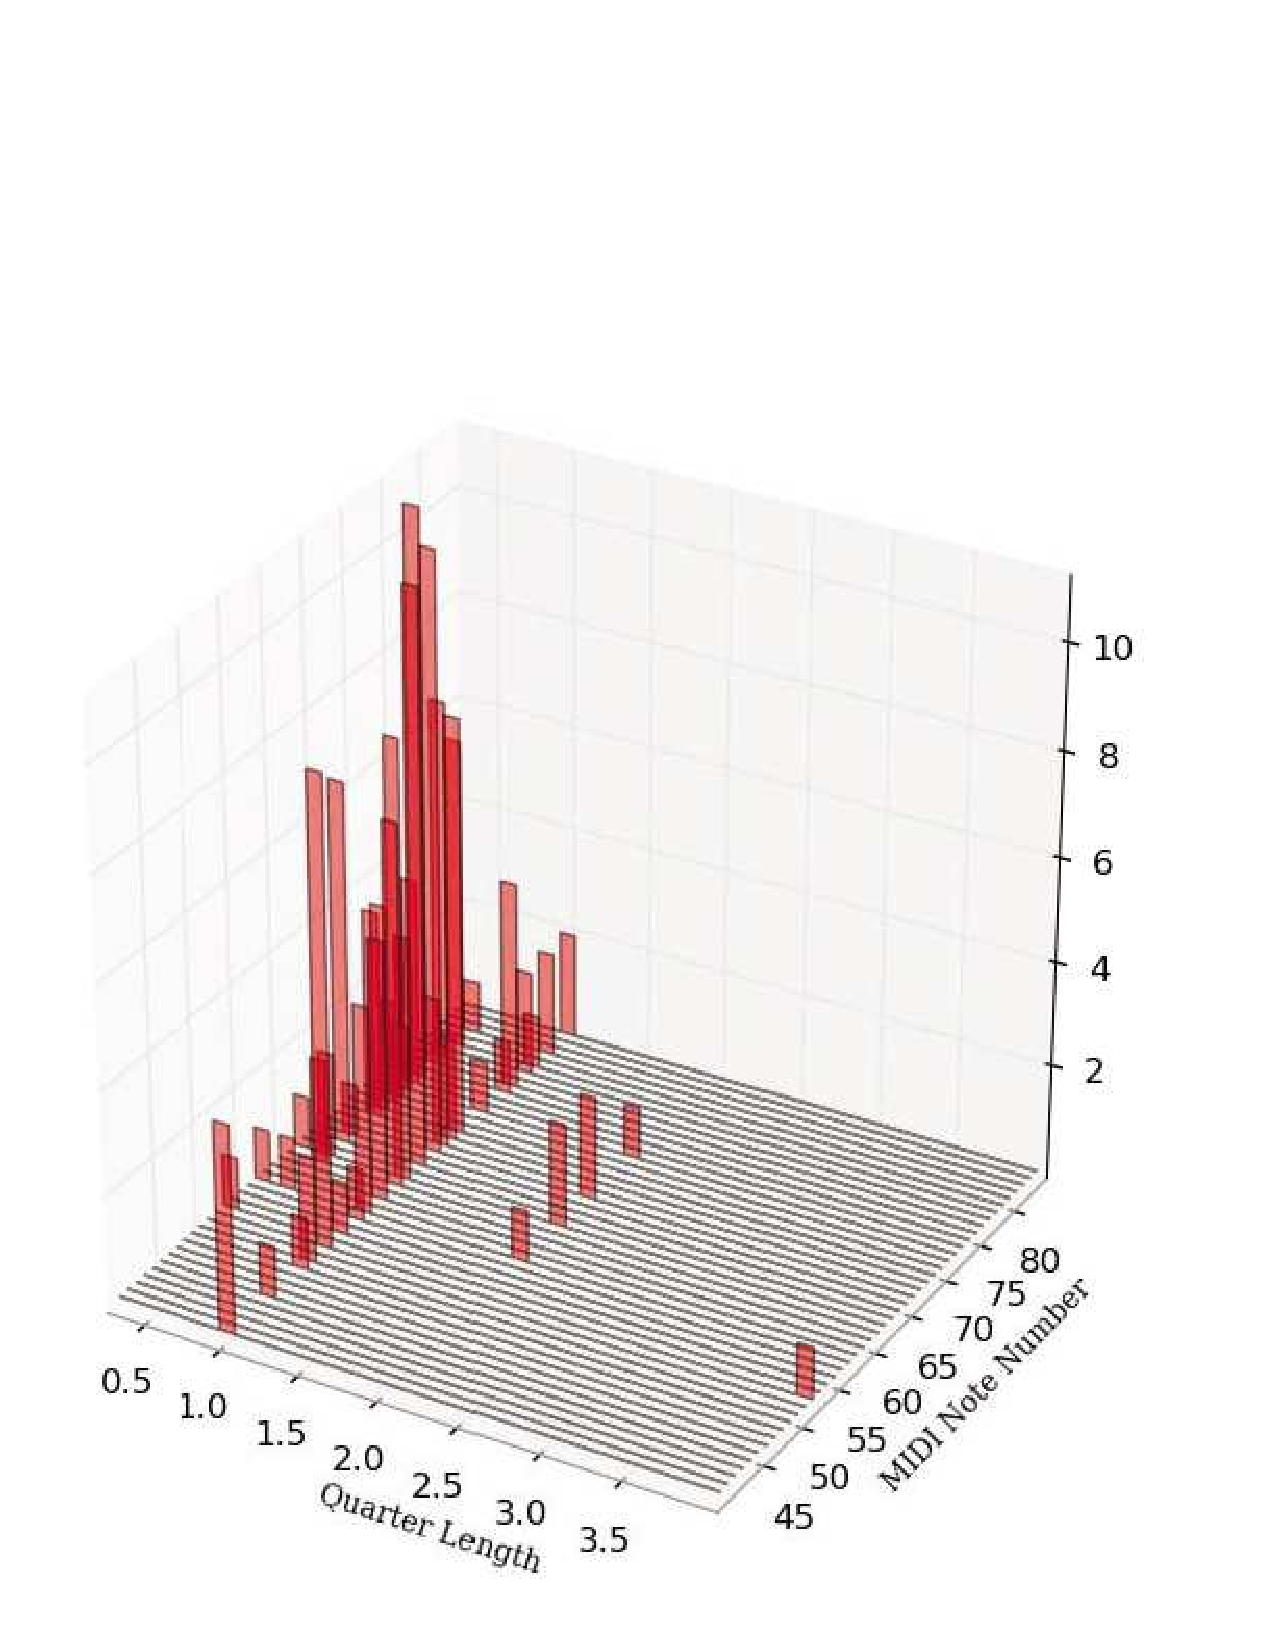
\includegraphics[width=0.8\textwidth, clip=true, trim = 15mm 10mm 20mm 70mm]{img/plot.pdf}
  \caption{Note Distribution by pitch and duration}
  \label{fig:note_distribution}
\end{figure}

The graph plots three features: pitch, duration of notes, and how frequently these pitches and
durations are used. It can be seen that pitches follow a type of bell-curve distribution, with few
high notes, few low notes, and many notes toward the middle of the register.  This line of inquiry
may reveal characteristics that are not easy to figure out, for instance, that a composer may be
following a certain trend.

\section{Summary}

With the \ac{DSL} \abcdt{} there is a considerable simplification of the process of creating an
\abcpt{} considering the following features:

\begin{itemize}
  \item It's not necessary to specify what doesn't need to be transformed (default functions);
  \item A transformation specification is rule-based which facilitates its writing;
  \item There's a set of rich \actuators{} which allows to precisely select a specific point to
  transform.
\end{itemize}

Using a structured processing of \abc{} allows an \abcpt{} to be described in an effective way.

Using Perl as the language embedded into \abcdt{} provides a rich environment to allow easy
processing of text. Furthermore, through the use of data structures, like hashes, the user has
bigger expressive power to specify transformations.\\

The next chapter presents some \abcpt{}s created using \abcdt{}.
